\documentclass[../../main]{subfiles}

\renewcommand\thesection{\arabic{section}}


\begin{document}

\section{Insulating Layer} \label{sec:}

The insides of the incubator needs to be isolated from the surroundings.
Otherwise thermal energy could leak in or leak out of the incubator and
ruin the cooling / heating capabilities of the incubator. So it is important
to thermally isolate the insides of the incubator where the seeds are sown.
See table \ref{tbl:partsNeedThermalInsulation} for the areas and parts that requires
thermal insulation.

\begin{center}
    \begin{tabularx} {\textwidth} {
            >{\centering \arraybackslash}X
            >{\centering \arraybackslash}X
        }

        \toprule

        Incubator Area & Exhaust System \\ \midrule

        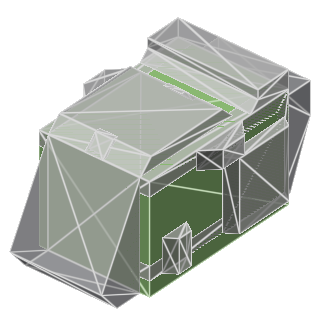
\includegraphics[
            height = 0.2\textheight,
        ] {
            pics/inc_area_right.png
        }

        &

        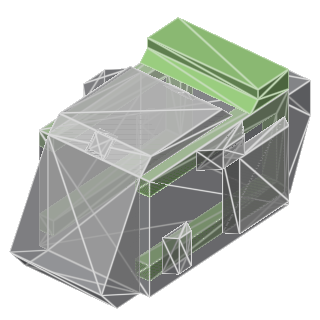
\includegraphics[
            height = 0.2\textheight,
        ] {
            pics/ext_right.png
        }

        \\ \midrule

        Top Hatch & Side Hatch \\ \midrule

        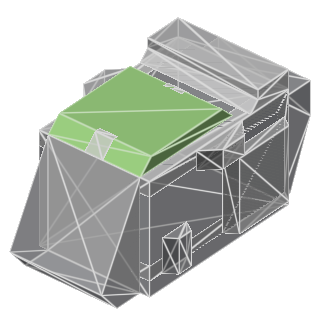
\includegraphics[
            height = 0.2\textheight,
        ] {
            pics/top_hatch_right.png
        }

        &

        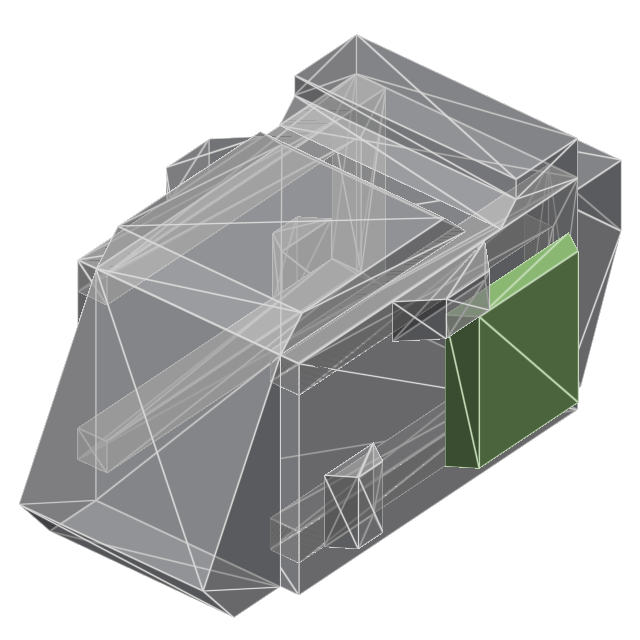
\includegraphics[
            height = 0.2\textheight,
        ] {
            pics/side_hatch_right.png
        }

        \\

        \bottomrule

    \end{tabularx}

    \captionof{table}{Incubator areas and parts that needs thermal insulation.}
    \label{tbl:partsNeedThermalInsulation}
\end{center}


As we can see from table \ref{tbl:partsNeedThermalInsulation}, the entire exhaust system is
needed to be thermally insulated. So the material we need to pick should be workable. PVC
foam is a good candidate. It has good insulating property and easily workable.


\end{document}
